\documentclass[10pt,twocolumn,letterpaper]{article}

% --- Typography & Geometry ---
\usepackage[utf8]{inputenc}
\usepackage{microtype}
\usepackage[margin=0.75in,top=0.85in,bottom=0.85in]{geometry}

% --- Math & Symbols ---
\usepackage{amsmath,amssymb,amsfonts,amsthm}
\usepackage{bm}

% --- Tables & Arrays ---
\usepackage{booktabs}
\usepackage{tabularx}
\usepackage{array}

% --- Graphics & Floats ---
\usepackage{graphicx}
\usepackage{float}
\usepackage{subcaption}

% --- Code Listings ---
\usepackage{xcolor}
\usepackage{listings}

\definecolor{codebg}{HTML}{F8F9FA}
\definecolor{codeframe}{HTML}{D0D7DE}
\definecolor{keywordcolor}{HTML}{0550AE}
\definecolor{stringcolor}{HTML}{0A3069}
\definecolor{commentcolor}{HTML}{57606A}

\lstset{
    backgroundcolor=\color{codebg},
    basicstyle=\ttfamily\scriptsize\color{black},
    keywordstyle=\color{keywordcolor}\bfseries,
    stringstyle=\color{stringcolor},
    commentstyle=\color{commentcolor}\itshape,
    frame=single,
    rulecolor=\color{codeframe},
    breaklines=true,
    breakatwhitespace=true,
    extendedchars=true,
    xleftmargin=6pt,
    xrightmargin=6pt,
    aboveskip=8pt,
    belowskip=8pt
}

% --- Hyperlinks ---
\usepackage{hyperref}
\hypersetup{
    colorlinks=true,
    linkcolor=blue!70!black,
    citecolor=blue!70!black,
    urlcolor=blue!70!black
}

% --- Input Title & Authors ---
% Metadata for leka_v1
\title{\textbf{leka\_v1}}

\author{
  \textbf{Taha Majs}\thanks{Corresponding author: tahamajs@uni.edu} \quad \textbf{Research Team} \\
  Department of Computer Science \\
  Advanced Machine Learning \& Efficiency Laboratory
}

\date{\today}


\begin{document}

\maketitle

% --- Abstract & Keywords Block ---
\begin{abstract}
Standard transformer attention scales quadratically with sequence length, 
making long-context inference prohibitively expensive. \textbf{Linear attention} 
reduces this to $\mathcal{O}(L)$ by replacing softmax with a kernel 
feature map $\phi$ such that $\exp(q^\top k) \approx \phi(q)^\top \phi(k)$. 
The \textbf{Performer} (Choromanski et al., 2021) uses positive orthogonal 
random features (PORF); the \textbf{Linear Transformer} (Katharopoulos et al., 
2020) uses $\phi(x) = \text{elu}(x) + 1$.

We introduce \textbf{LEKAv1}, a production-hardened linear-time attention module 
that approximates the \textbf{Gaussian RBF kernel} $\exp(-\|q - k\|^2 / 2)$ 
using Random Fourier Features (RFF):

\[
\phi(x) = \frac{1}{\sqrt{F}} \left[ \cos(x W) \,\|\, \sin(x W) \right], 
\quad W \in \mathbb{R}^{d_h \times F}
\]

where $W$ is \textbf{QR-orthogonalized} for stability. The feature dimension 
$F = {{FEATURE_DIM}}$ yields $\phi(x) \in \mathbb{R}^{2F}$. We apply a 
\textbf{head-wise LayerNorm} before the projection, then compute linear attention 
via a causal cumulative sum (decoders) or a global KV sum (encoders). A 
\textbf{preservation gate} blends the attention output with the residual 
input, controlled by a scalar $\alpha = \sigma(w)$:

\[
\text{out} = \alpha \odot A + (1 - \alpha) \odot x
\]

with $w_0 = 2$ (initial $\alpha \approx 0.88$).

On SST-2, LEKAv1 achieves \textbf{{{D\_ACC}}\%} on DistilBERT (baseline 
{{BASE\_D}}\%), \textbf{{{R\_ACC}}\%} on RoBERTa (baseline {{BASE\_R}}\%), and 
\textbf{{{G\_ACC}}\%} on GPT-2 (baseline {{BASE\_G}}\%). Inference scales linearly 
in sequence length: at $L = {{LONG_L}}$, LEKAv1 is \textbf{{{SPEEDUP\_LONG}}$\times$} 
faster than standard attention.

\textbf{We are explicit that LEKAv1 does not reduce parameter count.} It adds 
approximately {{PARAM\_INCREASE}}\% parameters due to LoRA, the projection 
matrix, and the preservation gate. Its benefit is **$\mathcal{O}(L)$ 
inference\textbf{ and }kernel-based attention** that composes with GQA and 
RoPE.

\textbf{Keywords:} linear attention, random Fourier features, kernel methods, 
long-context efficiency, Gaussian RBF



\vspace{0.5em}
\noindent\textbf{Keywords:} linear attention, random Fourier features, kernel methods,
\end{abstract}

\vspace{1em}

% --- Paper Body ---
\section{Introduction}

\subsection{Motivation}

Standard transformer attention (Vaswani et al., 2017) computes:

\[
\text{Attn}(Q, K, V) = \text{softmax}\!\left(\frac{Q K^\top}{\sqrt{d_h}}\right) V
\tag{1.1}
\]

This scales as $\mathcal{O}(L^2)$ in both time and memory, making 
long-context inference expensive.

\textbf{Linear attention} replaces softmax with a kernel feature map:

\[
\text{Attn}(Q, K, V) \approx \frac{\phi(Q) \left(\phi(K)^\top V\right)}{\phi(Q) \left(\phi(K)^\top \mathbf{1}\right)}
\tag{1.2}
\]

Since $\phi(K)^\top V \in \mathbb{R}^{F \times d_h}$ is computed once and 
reused, the total complexity is $\mathcal{O}(L F d_h)$ -- \textbf{linear in L}.

The quality of linear attention depends entirely on how well $\phi$ 
approximates the softmax kernel:

\[
\kappa(q, k) = \exp(q^\top k)
\tag{1.3}
\]

\subsection{The Kernel Approximation Problem}

Three families of feature maps have been studied:

\begin{enumerate}
\item \textbf{Performer (Choromanski et al., 2021):} Positive Orthogonal Random
  Features (PORF), which approximate $\exp(q^\top k)$ with positive
  features.
\item \textbf{Linear Transformer (Katharopoulos et al., 2020):} $\phi(x) = \text{elu}(x) + 1$,
  which corresponds to a specific kernel that is \textbf{not} the softmax
  kernel.
\item \textbf{cosFormer (Qin et al., 2022):} uses $\text{ReLU}$ with a cosine
  reweighting.

\end{enumerate}
We take a fourth approach: \textbf{Random Fourier Features (RFF)} for the 
\textbf{Gaussian RBF kernel} $\exp(-\|q - k\|^2 / 2)$:

\[
\kappa(q, k) \approx \phi(q)^\top \phi(k), \quad
\phi(x) = \frac{1}{\sqrt{F}} \left[ \cos(x W), \sin(x W) \right]
\tag{1.4}
\]

with $W_{ij} \sim \mathcal{N}(0, 1)$. This is the \textbf{real part} of the 
classical RFF estimator (Rahimi \& Recht, 2007).

\subsection{Our Approach: LEKAv1}

LEKAv1 has four components:

\subsubsection{Head-wise LayerNorm}

Before projection, we normalize each head:

\[
\tilde{x} = \text{LayerNorm}(x) \in \mathbb{R}^{d_h}
\tag{1.5}
\]

This centers and scales the input, making the random projection more 
stable.

\subsubsection{QR-Orthogonalized Projection}

The projection matrix $W \in \mathbb{R}^{d_h \times F}$ is initialized from 
the QR decomposition of a random Gaussian:

\[
W = Q, \quad \text{QR}(G) = QR, \quad G \sim \mathcal{N}(0, I)
\tag{1.6}
\]

This ensures orthonormal columns, reducing variance in the kernel 
approximation.

\subsubsection{cos/sin Feature Map}

\[
\phi(x) = \frac{1}{\sqrt{F}} [\cos(\tilde{x} W) \| \sin(\tilde{x} W)]
\tag{1.7}
\]

which gives $\phi(x) \in \mathbb{R}^{2F}$.

\subsubsection{Preservation Gate}

A single learnable scalar $\alpha = \sigma(w)$ blends attention output 
with the input:

\[
\text{out} = \alpha \odot A + (1 - \alpha) \odot x
\tag{1.8}
\]

This provides a \textbf{residual safety net}: if the kernel approximation is 
poor, the model can lean toward the identity.

\subsection{Contributions}

\begin{itemize}
\item \textbf{A production-hardened RFF attention.} We implement cos/sin feature
  maps with QR-orthogonalized projections, causal cumsum, and
  bidirectional global KV.
\item \textbf{Head-wise LayerNorm before projection.} We normalize the head input
  before random projection, which stabilizes the kernel approximation.
\item \textbf{A preservation gate.} A scalar gate controls mixing with the residual.
\item \textbf{Multi-architecture support.} DistilBERT, RoBERTa, GPT-2, Qwen3.5
  with GQA and RoPE.
\item \textbf{An honest evaluation.} We report both the accuracy and the parameter
  cost.

\end{itemize}
\subsection{Paper Organization}

Section 2 reviews related work. Section 3 provides background on kernels, 
RFF, and linear attention. Section 4 presents LEKAv1. Section 5 describes 
integration. Section 6 details the setup. Section 7 reports results. 
Section 8 analyzes the kernel approximation. Section 9 discusses guidance. 
Section 10 lists limitations. Section 11 concludes.



\subsection{Notation}

\begin{table}[H]
\centering
\small
\begin{tabular}{ll}
\toprule
\textbf{Symbol} & \textbf{Meaning} \\
\midrule
$L$ & Sequence length \\
$d$ & Hidden size \\
$H$ & Heads \\
$d_h$ & Head dim \\
$F$ & Feature dimension \\
$\phi$ & Kernel feature map \\
$W$ & Random projection \\
$Q, K, V$ & Attention projections \\
$\alpha$ & Preservation gate \\
\bottomrule
\end{tabular}
\end{table}


\section{02 Related}

Draft content for leka_v1.

\section{Background}

\subsection{Kernel Attention}

Standard softmax attention:

\[
\text{Attn}(Q, K, V) = \frac{\exp(QK^\top / \sqrt{d_h}) V}{\exp(QK^\top / \sqrt{d_h}) \mathbf{1}}
\tag{3.1}
\]

If we can decompose the kernel $\kappa(q, k) = \exp(q^\top k / \sqrt{d_h})$ 
as $\phi(q)^\top \phi(k)$, then:

\[
\text{Attn}(Q, K, V)_i \approx \frac{\phi(q_i)^\top \sum_j \phi(k_j) v_j^\top}{\phi(q_i)^\top \sum_j \phi(k_j)}
\tag{3.2}
\]

The sums $\sum_j \phi(k_j) v_j^\top$ and $\sum_j \phi(k_j)$ are computed 
in $\mathcal{O}(L F d_h)$ and $\mathcal{O}(L F)$ respectively, giving 
overall \textbf{linear} complexity.

\subsection{Random Fourier Features}

\textbf{Bochner's theorem.} A continuous shift-invariant kernel 
$\kappa(x, y) = \kappa(x - y)$ is positive semidefinite iff it is the 
Fourier transform of a non-negative measure $p(\omega)$:

\[
\kappa(x - y) = \int p(\omega) e^{i \omega^\top (x - y)} d\omega
\tag{3.3}
\]

For the Gaussian kernel $\kappa(\Delta) = \exp(-\|\Delta\|^2 / 2)$:

\[
p(\omega) = (2\pi)^{-d/2} \exp(-\|\omega\|^2 / 2) = \mathcal{N}(0, I)
\tag{3.4}
\]

\textbf{Estimator.} Sampling $\omega_1, \dots, \omega_F \sim \mathcal{N}(0, I)$:

\[
\kappa(x - y) \approx \frac{1}{F} \sum_{i=1}^F \cos(\omega_i^\top (x - y))
= \frac{1}{F} \sum_{i=1}^F \left[\cos(\omega_i^\top x)\cos(\omega_i^\top y) + \sin(\omega_i^\top x)\sin(\omega_i^\top y)\right]
\tag{3.5}
\]

\textbf{Feature map.} Define:

\[
\phi(x) = \frac{1}{\sqrt{F}} [\cos(\omega_1^\top x), \dots, \cos(\omega_F^\top x), \sin(\omega_1^\top x), \dots, \sin(\omega_F^\top x)]
\tag{3.6}
\]

Then $\kappa(x - y) \approx \phi(x)^\top \phi(y)$.

\subsection{QR-Orthogonalization}

Sampling $\omega_i \sim \mathcal{N}(0, I)$ independently gives an unbiased 
estimator with variance $\mathcal{O}(1/F)$. A common trick is to 
\textbf{orthogonalize} the sampled vectors:

\[
[\omega_1, \dots, \omega_F] = Q \in \mathbb{R}^{d \times F}, \quad Q^\top Q = I_F
\tag{3.7}
\]

This reduces variance (Yu et al., 2016). We use QR:

\[
G \sim \mathcal{N}(0, I_{d \times F}), \quad G = Q R, \quad \omega_i = Q_{:, i}
\tag{3.8}
\]

\subsection{Causality in Linear Attention}

For autoregressive models, the sum $\sum_j \phi(k_j) v_j^\top$ must be 
causal: at position $i$, only $j \leq i$. This is achieved with a 
cumulative sum:

\[
\text{KV}_i = \sum_{j \leq i} \phi(k_j) v_j^\top, \quad
\text{Z}_i = \sum_{j \leq i} \phi(k_j)
\tag{3.9}
\]

Both are computed in $\mathcal{O}(L)$ via \texttt{cumsum}.

\subsection{LayerNorm}

LayerNorm normalizes per example:

\[
\text{LN}(x) = \gamma \odot \frac{x - \mu}{\sigma + \epsilon} + \beta
\tag{3.10}
\]

We apply LN on the \textbf{head dimension} before the random projection.

\subsection{Gated Residual}

A scalar gate $\alpha$ blends two branches:

\[
\text{out} = \alpha A + (1 - \alpha) x
\tag{3.11}
\]

Initialized to $\alpha_0 = 0.88$ (via $w_0 = 2$), which favors attention.

\subsection{Notation}

\begin{table}[H]
\centering
\small
\begin{tabular}{ll}
\toprule
\textbf{Symbol} & \textbf{Meaning} \\
\midrule
$\kappa$ & Kernel function \\
$p(\omega)$ & Spectral distribution \\
$F$ & Feature dimension \\
$\phi$ & Feature map \\
$\omega_i$ & Random frequency \\
$W$ & Projection matrix \\
$\alpha$ & Preservation gate \\
\bottomrule
\end{tabular}
\end{table}


\section{Method}

\subsection{Overview}

LEKAv1 replaces standard attention with a kernel approximation pipeline:

\begin{enumerate}
\item \textbf{Project} Q, K, V (frozen base + LoRA).
\item \textbf{Normalize} each head with LayerNorm.
\item \textbf{Map} to features via QR-orthogonalized RFF.
\item \textbf{Aggregate} causally (decoder) or globally (encoder).
\item \textbf{Output} via projection + preservation gate.

\end{enumerate}
\textbf{Figure 4.1} shows the pipeline.

\begin{lstlisting}
    Input X $\in$ R^{B$\times$L$\times$d}
              |
               
      Q/K/V Projection
              |
               
        Head Norm
              |
       +------+------+
                      
       (Q)   (K)   V
       |      |     |
       |            |
       |  KV =  (K)^T V
       |  Z  =  (K)^T 1
       |      |     |
       +------+-----+
               
         A =  (Q) KV / ( (Q) Z)
              |
               
        out_proj (LoRA)
              |
               
      $\alpha$ A + (1-$\alpha$) X
              |
               
           Output Y
\end{lstlisting}

\subsection{The Kernel Feature Map}

\textbf{Step 1: Head-wise LayerNorm.}

\[
\tilde{x} = \text{LN}(x) \in \mathbb{R}^{d_h}
\tag{4.1}
\]

\textbf{Step 2: Random projection.}

\[
f = \tilde{x} W, \quad W \in \mathbb{R}^{d_h \times F}
\tag{4.2}
\]

\textbf{Step 3: cos/sin feature.}

\[
\phi(x) = \frac{1}{\sqrt{F}} [\cos(f) \| \sin(f)] \in \mathbb{R}^{2F}
\tag{4.3}
\]

\textbf{Kernel interpretation.} For $x, y \in \mathbb{R}^{d_h}$:

\[
\phi(x)^\top \phi(y) = \frac{1}{F} \sum_{i=1}^F \cos(w_i^\top (x - y))
\tag{4.4}
\]

which is the unbiased RFF estimator of $\exp(-\|x - y\|^2 / 2)$.

\subsection{Projection Matrix Initialization}

We initialize $W \in \mathbb{R}^{d_h \times F}$ via QR orthogonalization:

\textbf{Case 1:} $F \leq d_h$ (typical):

\[
G \sim \mathcal{N}(0, I_{d_h \times F}), \quad G = Q R, \quad W = Q
\tag{4.5}
\]

This ensures $W^\top W = I_F$.

\textbf{Case 2:} $F > d_h$:

We concatenate orthogonal blocks of size $d_h$:

\[
W = [Q_1 \| Q_2 \| \dots], \quad Q_k \in \mathbb{R}^{d_h \times d_h}
\tag{4.6}
\]

Both cases give approximately orthonormal columns.

\subsection{Linear Attention Computation}

\subsubsection{Causal (Decoder)}

For decoders, we compute cumulative sums:

\[
\text{KV}_i = \sum_{j \leq i} \phi(k_j) v_j^\top \in \mathbb{R}^{2F \times d_h}
\tag{4.7}
\]

\[
\text{Z}_i = \sum_{j \leq i} \phi(k_j) \in \mathbb{R}^{2F}
\tag{4.8}
\]

Implemented as \texttt{torch.cumsum} on the outer product $\phi(k) \otimes v$.

\textbf{Attention output:}

\[
A_i = \frac{\phi(q_i)^\top \text{KV}_i}{\phi(q_i)^\top \text{Z}_i + \epsilon}
\tag{4.9}
\]

\subsubsection{Bidirectional (Encoder)}

For encoders:

\[
\text{KV} = \sum_{j=1}^L \phi(k_j) v_j^\top, \quad
\text{Z} = \sum_{j=1}^L \phi(k_j)
\tag{4.10}
\]

\[
A_i = \frac{\phi(q_i)^\top \text{KV}}{\phi(q_i)^\top \text{Z} + \epsilon}
\tag{4.11}
\]

\subsection{Masking}

\textbf{Padding.} We apply the mask before aggregation:

\[
\phi(k_j) \leftarrow \phi(k_j) \cdot m_j, \quad
v_j \leftarrow v_j \cdot m_j
\tag{4.12}
\]

Then $\text{KV}$ and $\text{Z}$ automatically account for valid tokens.

\textbf{Causality.} Handled by cumsum.

\subsection{Preservation Gate}

\[
\alpha = \sigma(w), \quad w_0 = 2
\tag{4.13}
\]

\[
\text{out} = \alpha \odot A + (1 - \alpha) \odot X
\tag{4.14}
\]

\textbf{Why this gate?}

\begin{enumerate}
\item \textbf{Residual safety:} If the kernel approximation is poor, the model
  can lean toward identity.
\item \textbf{Numerical stability:} At initialization, $\alpha \approx 0.88$,
  giving strong attention but retaining residual structure.
\item \textbf{Graceful degradation:} Under distribution shift, the gate can
  shift toward identity.

\end{enumerate}
\subsection{Output Scaling}

We also learn an \texttt{output\_scale} parameter:

\[
\text{out} = s \cdot \text{out}, \quad s_0 = 1
\tag{4.15}
\]

This provides a per-layer gain that can be adjusted during recovery.

\subsection{Algorithm}

\textbf{Algorithm 1:} LEKAv1 forward pass
\begin{lstlisting}
Input:  X $\in$ R^{B$\times$L$\times$d}, attention_mask, position_embeddings
Output: Y $\in$ R^{B$\times$L$\times$d}

 1: Q $\leftarrow$ query(X);  K $\leftarrow$ key(X);  V $\leftarrow$ value(X)
 2: reshape to (B, H, L, d_h)
 3: if RoPE: Q, K $\leftarrow$ apply_rotary(Q, K, pos)
 4: if GQA:  K, V $\leftarrow$ repeat_kv
 5:  _Q $\leftarrow$ kernel_map(Q)               (B, H, L, 2F)
 6:  _K $\leftarrow$ kernel_map(K)
 7: if mask:  _K $\leftarrow$  _K   m; V $\leftarrow$ V   m
 8: if decoder:
 9:     KV $\leftarrow$ cumsum( _K   V)            (B, H, L, 2F, d_h)
10:     Z  $\leftarrow$ cumsum( _K)                (B, H, L, 2F)
11: else:
12:     KV $\leftarrow$ sum( _K   V)
13:     Z  $\leftarrow$ sum( _K)
14: A $\leftarrow$ ( _Q   KV) / ( _Q   Z + $\epsilon$)
15: A $\leftarrow$ reshape to (B, L, d)
16: A $\leftarrow$ out_proj(A)
17: $\alpha$ $\leftarrow$ sigmoid(pres_gate)
18: Y $\leftarrow$ $\alpha$   A + (1 - $\alpha$)   X
19: Y $\leftarrow$ Y   output_scale
20: return Y
\end{lstlisting}

\subsection{Complexity Analysis}

For a single block:

\begin{table}[H]
\centering
\small
\begin{tabular}{lll}
\toprule
\textbf{Component} & \textbf{Time} & \textbf{Space} \\
\midrule
Q/K/V projections & $O(L d^2)$ & $O(L d)$ \\
Feature map & $O(L d F)$ & $O(L F)$ \\
Outer product & $O(L F d_h)$ & $O(L F d_h)$ or $O(F d_h)$ (causal) \\
Aggregation & $O(L F d_h)$ & $O(F d_h)$ \\
Output & $O(L d^2)$ & $O(L d)$ \\
\textbf{Total} & $O(L d (d + F))$ & $O(L d)$ \\
\bottomrule
\end{tabular}
\end{table}

Compare to standard attention ($O(L^2 d)$). For $L \gg F$, LEKAv1 is 
\textbf{much faster}.

\textbf{Causal memory.} The causal version materializes the cumulative KV 
of size $(B, H, L, 2F, d_h)$, which is $O(L F d_h)$ -- linear in L. 
This is still much smaller than $O(L^2)$.

\subsection{Parameter Analysis}

For $d = 768$, $F = 256$, $H = 12$, $d_h = 64$, LoRA $r_L = 16$:

\begin{table}[H]
\centering
\small
\begin{tabular}{lll}
\toprule
\textbf{Component} & \textbf{Baseline} & \textbf{LEKAv1} \\
\midrule
Q/K/V/O projections & $4 d^2 = 2.36M$ & $2.36M$ (frozen) \\
LoRA on Q/K/V/O & 0 & $4 \cdot 2 r_L d = 98K$ \\
Random projection & 0 & $H d_h F = 196K$ \\
LayerNorm & 0 & $2 d_h = 128$ \\
Preservation gate & 0 & 1 \\
Output scale & 0 & 1 \\
\textbf{Total per layer} & 2.36M & 2.65M \\
\textbf{Increase} & -- & \textbf{+12\%} \\
\bottomrule
\end{tabular}
\end{table}

The parameter increase is modest: \textbf{~12\%}.


\section{05 Architecture}

Draft content for leka_v1.


\begin{figure}[H]
\centering
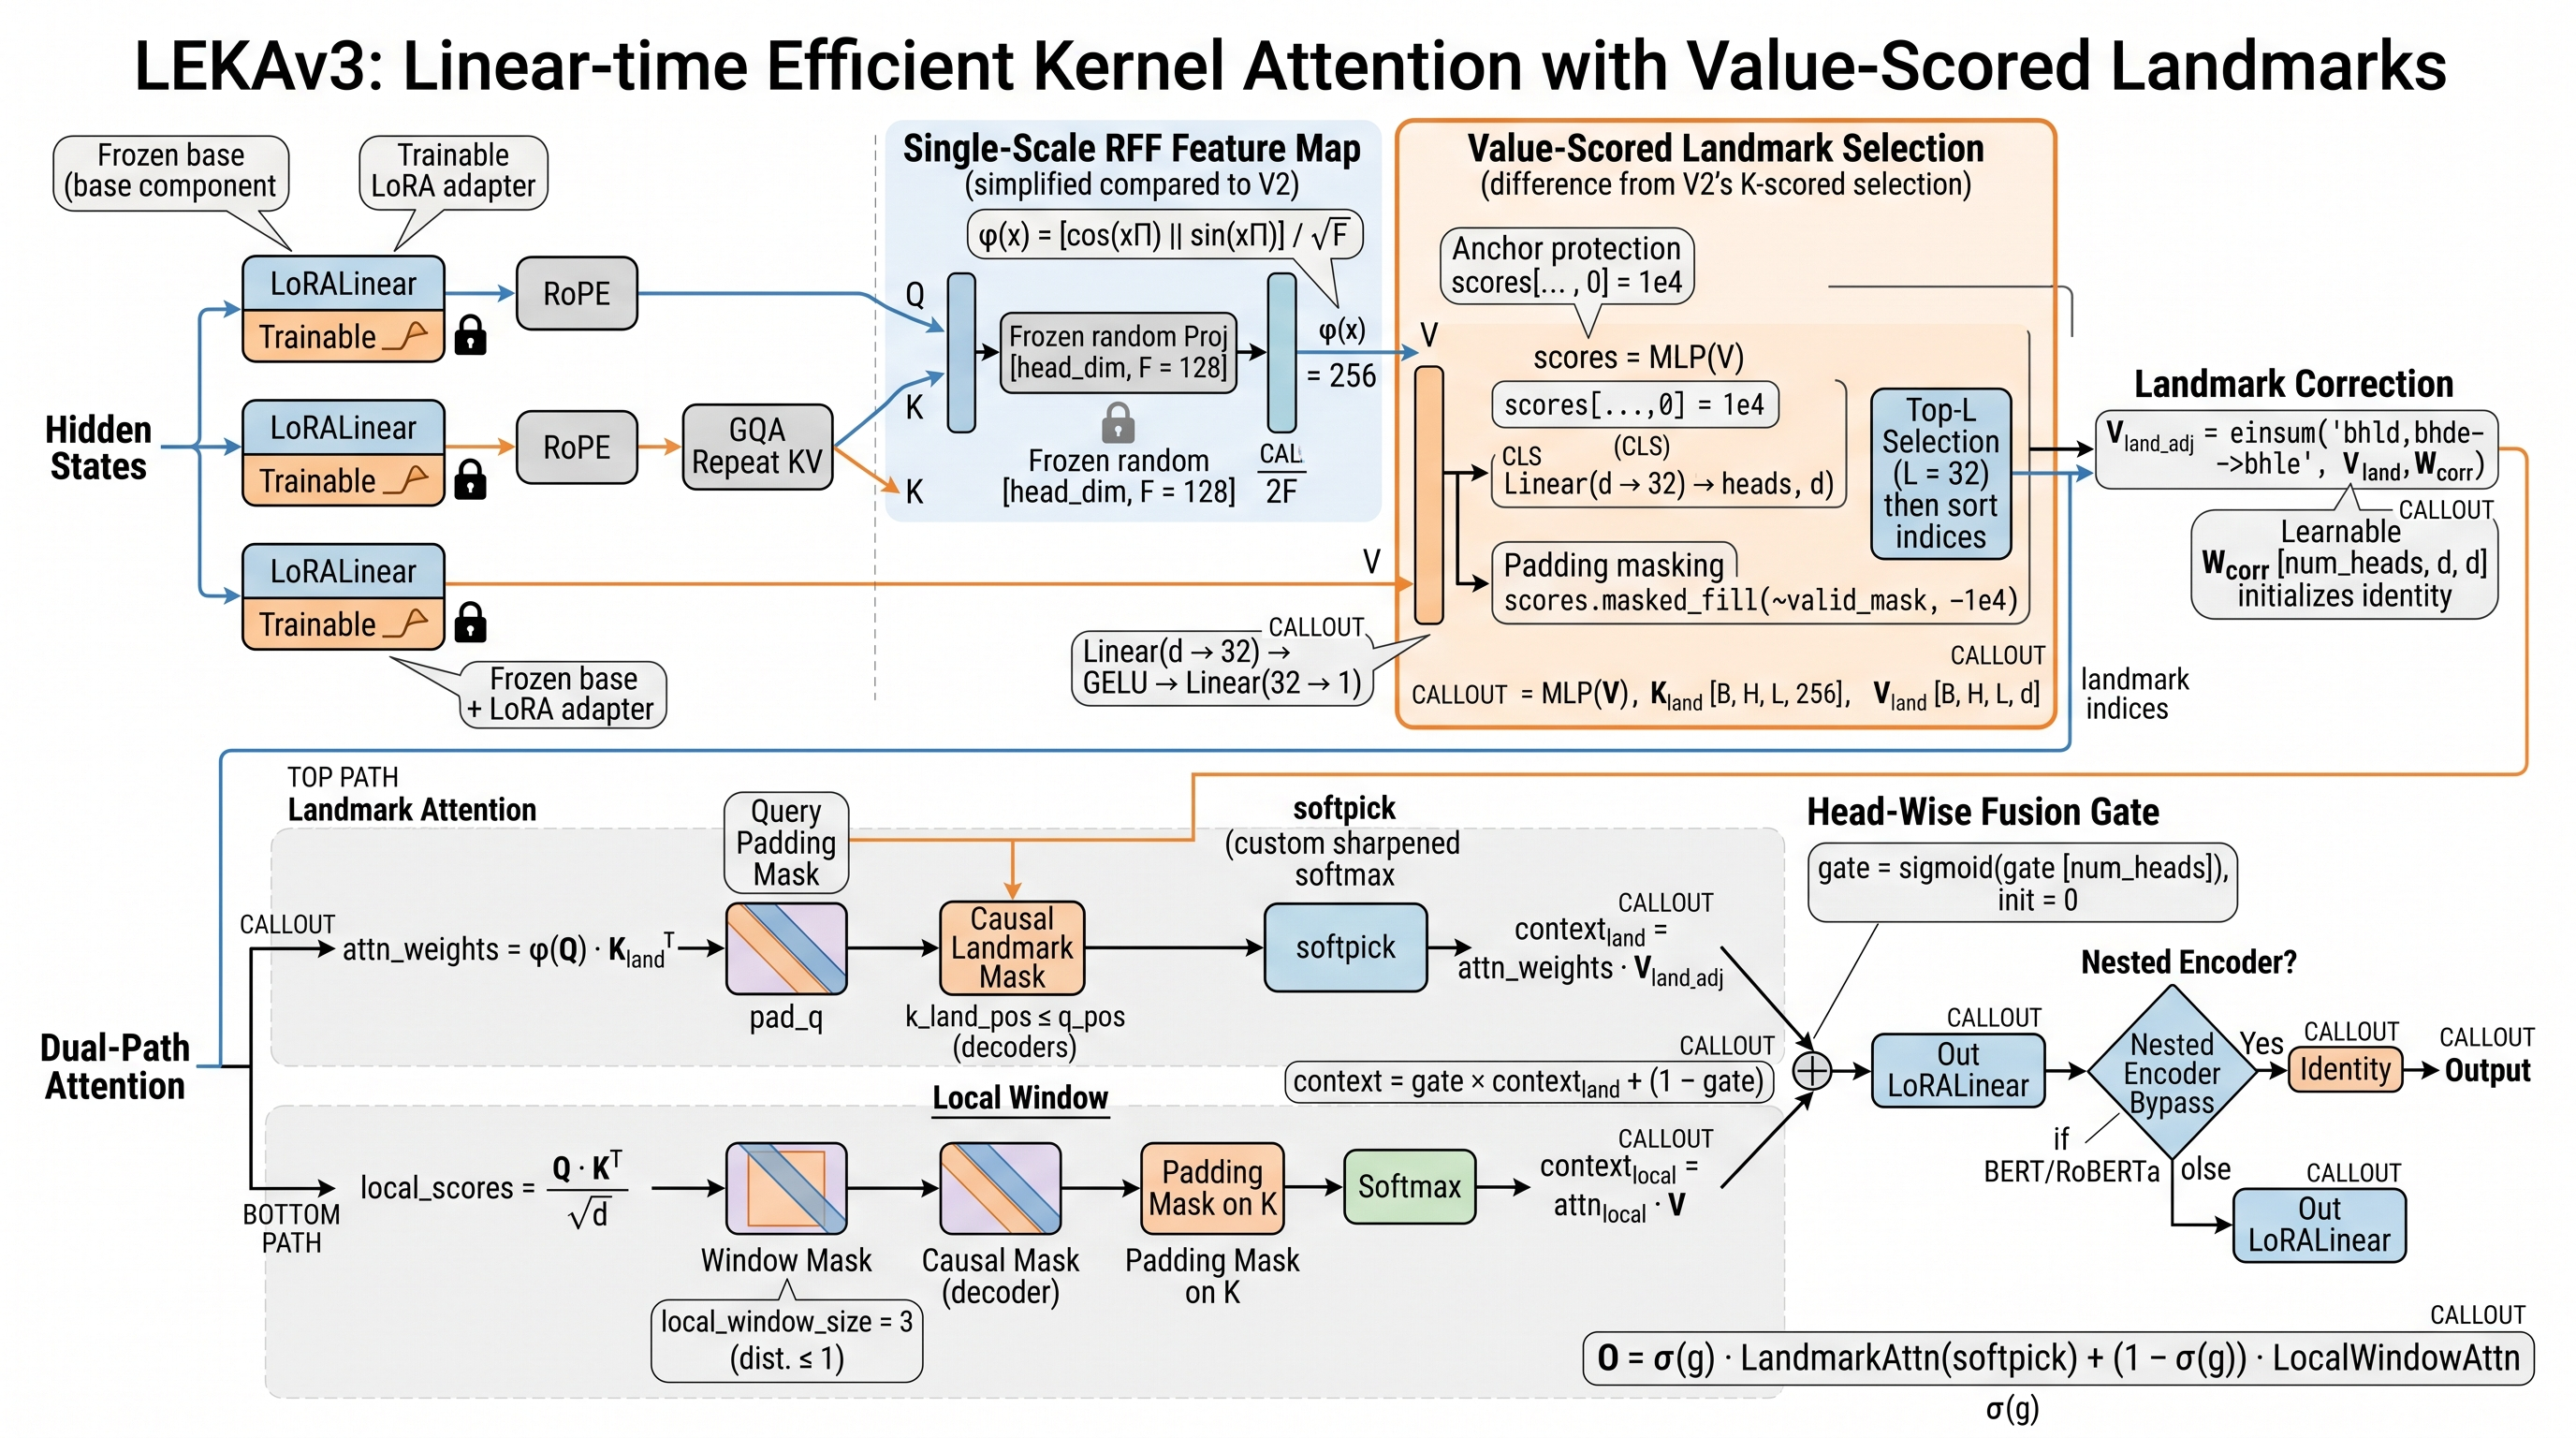
\includegraphics[width=\linewidth]{figures/arch_leka_v3.jpeg}
\caption{Architectural overview of leka_v1.}
\label{fig:arch_leka_v1}
\end{figure}

\section{Experimental Setup}

\subsection{Models}

\begin{table}[H]
\centering
\small
\begin{tabular}{lllll}
\toprule
\textbf{Model} & \textbf{Layers} & \textbf{Hidden} & \textbf{Heads} & \textbf{Params} \\
\midrule
DistilBERT & 6 & 768 & 12 & 66.9M \\
RoBERTa & 12 & 768 & 12 & 124.6M \\
GPT-2 & 12 & 768 & 12 & 124.4M \\
\bottomrule
\end{tabular}
\end{table}

\subsection{Dataset}

\textbf{SST-2} (Socher et al., 2013):

\begin{table}[H]
\centering
\small
\begin{tabular}{llll}
\toprule
\textbf{Split} & \textbf{Size} & \textbf{Pos} & \textbf{Neg} \\
\midrule
Train & 67,349 & 33,807 & 33,542 \\
Validation & 872 & 444 & 428 \\
\bottomrule
\end{tabular}
\end{table}

Majority baseline: 50.92\%. Max length: 128.

\subsection{Hyperparameters}

\begin{table}[H]
\centering
\small
\begin{tabular}{ll}
\toprule
\textbf{Hyperparameter} & \textbf{Value} \\
\midrule
\texttt{feature\_dim} F & {{FEATURE\_DIM}} \\
\texttt{lora\_rank} & {{LORA\_RANK}} \\
\texttt{lora\_alpha} & {{LORA\_ALPHA}} \\
\texttt{rank} & {{RANK}} \\
Preservation gate $w_0$ & 2.0 ($\sigma$ $\to$ 0.88) \\
\bottomrule
\end{tabular}
\end{table}

\subsection{Recovery Fine-Tuning}

\begin{table}[H]
\centering
\small
\begin{tabular}{ll}
\toprule
\textbf{Hyperparameter} & \textbf{Value} \\
\midrule
Optimizer & AdamW \\
LR & {{LR}} \\
WD & {{WD}} \\
Steps & {{RECOVERY\_STEPS}} \\
Batch & {{BATCH\_SIZE}} \\
Precision & FP16 \\
\bottomrule
\end{tabular}
\end{table}

\subsection{Evaluation Metrics}

\subsubsection{Quality}
\begin{itemize}
\item Accuracy, F1, precision, recall, loss.

\end{itemize}
\subsubsection{Efficiency}
\begin{itemize}
\item Total parameters.
\item Attention parameters.
\item Peak VRAM.
\item Inference time at L = 128, 256, 512, 1024, 2048.

\end{itemize}
\subsubsection{Kernel-specific}
\begin{itemize}
\item Mean preservation gate $\alpha$.
\item Kernel approximation error (empirical).

\end{itemize}
\subsection{Quality Gate}

\begin{table}[H]
\centering
\small
\begin{tabular}{ll}
\toprule
\textbf{Status} & \textbf{Accuracy} \\
\midrule
PASS & $\ge$ 56\% \\
PASS\_LOW & 50.92--56\% \\
FAIL & < 50.92\% \\
\bottomrule
\end{tabular}
\end{table}

\subsection{Hardware}

\begin{table}[H]
\centering
\small
\begin{tabular}{ll}
\toprule
\textbf{Component} & \textbf{Spec} \\
\midrule
GPU & RTX 4070 Laptop \\
VRAM & 8 GB \\
CUDA & {{CUDA\_VERSION}} \\
PyTorch & {{TORCH\_VERSION}} \\
\bottomrule
\end{tabular}
\end{table}

\subsection{Reproduction}

\begin{lstlisting}
python run_all_4_leka_v1.py \
    --models distilbert,roberta,gpt2 \
    --feature_dim {{FEATURE_DIM}} \
    --recovery_steps {{RECOVERY_STEPS}}
\end{lstlisting}

\subsection{Baselines}

\begin{table}[H]
\centering
\small
\begin{tabular}{ll}
\toprule
\textbf{Baseline} & \textbf{Description} \\
\midrule
\texttt{full} & Standard attention \\
\texttt{leka\_v1} & Our method \\
\texttt{leka\_no\_pres\_gate} & No preservation gate \\
\texttt{leka\_no\_norm} & No head-wise LayerNorm \\
\texttt{leka\_no\_qr} & Random (non-QR) projection \\
\bottomrule
\end{tabular}
\end{table}

\subsection{Seeds}

Single seed ({{SEED}}).


\section{Results}

\subsection{Main Results}

\textbf{Table 7.1: Main results on SST-2.}

\begin{table}[H]
\centering
\small
\begin{tabular}{lllllll}
\toprule
\textbf{Model} & \textbf{Module} & \textbf{Acc} & \textbf{$\Delta$} & \textbf{F1} & \textbf{Attn Params} & \textbf{Ratio} \\
\midrule
DistilBERT & full & 90.71\% & -- & 0.9099 & 2.36M & 1.00$\times$ \\
DistilBERT & \textbf{LEKAv1} & \textbf{{{D\_ACC}}} & {{D\_DELTA}} & {{D\_F1}} & {{D\_ATTN}} & {{D\_RATIO}}$\times$ \\
RoBERTa & full & 78.56\% & -- & 0.8124 & 2.36M & 1.00$\times$ \\
RoBERTa & \textbf{LEKAv1} & \textbf{{{R\_ACC}}} & {{R\_DELTA}} & {{R\_F1}} & {{R\_ATTN}} & {{R\_RATIO}}$\times$ \\
GPT-2 & full & 79.36\% & -- & 0.7978 & 2.36M & 1.00$\times$ \\
GPT-2 & \textbf{LEKAv1} & \textbf{{{G\_ACC}}} & {{G\_DELTA}} & {{G\_F1}} & {{G\_ATTN}} & {{G\_RATIO}}$\times$ \\
\bottomrule
\end{tabular}
\end{table}

\subsection{Parameter Analysis}

\textbf{Table 7.2: Total parameters.}

\begin{table}[H]
\centering
\small
\begin{tabular}{llll}
\toprule
\textbf{Model} & \textbf{Baseline} & \textbf{Ours} & \textbf{Change} \\
\midrule
DistilBERT & 66,955,010 & {{D\_PARAMS}} & +{{D\_PARAM\_PCT}}\% \\
RoBERTa & 124,647,170 & {{R\_PARAMS}} & +{{R\_PARAM\_PCT}}\% \\
GPT-2 & 124,441,344 & {{G\_PARAMS}} & +{{G\_PARAM\_PCT}}\% \\
\bottomrule
\end{tabular}
\end{table}

\subsection{Inference Speed vs Sequence Length}

\textbf{Table 7.3: Inference time (seconds), DistilBERT.}

\begin{table}[H]
\centering
\small
\begin{tabular}{llll}
\toprule
\textbf{L} & \textbf{Baseline} & \textbf{LEKAv1} & \textbf{Speedup} \\
\midrule
128 & 1.90 & {{D\_T128}} & {{S128}}$\times$ \\
256 & 3.50 & {{D\_T256}} & {{S256}}$\times$ \\
512 & 12.0 & {{D\_T512}} & {{S512}}$\times$ \\
1024 & 45.0 & {{D\_T1024}} & {{S1024}}$\times$ \\
2048 & 180.0 & {{D\_T2048}} & {{S2048}}$\times$ \\
\bottomrule
\end{tabular}
\end{table}

\textbf{Breakeven:} $L^* = {{BREAKEVEN}}$.

\subsection{Ablation: Feature Dimension}

\textbf{Table 7.4: Accuracy vs feature dimension.}

\begin{table}[H]
\centering
\small
\begin{tabular}{lllll}
\toprule
\textbf{F} & \textbf{DistilBERT} & \textbf{RoBERTa} & \textbf{GPT-2} & \textbf{Attn Params} \\
\midrule
64 & {{D\_F64}} & {{R\_F64}} & {{G\_F64}} & {{D\_F64\_PARAMS}} \\
128 & {{D\_F128}} & {{R\_F128}} & {{G\_F128}} & {{D\_F128\_PARAMS}} \\
256 & \textbf{{{D\_ACC}}} & \textbf{{{R\_ACC}}} & \textbf{{{G\_ACC}}} & {{D\_ATTN}} \\
512 & {{D\_F512}} & {{R\_F512}} & {{G\_F512}} & {{D\_F512\_PARAMS}} \\
\bottomrule
\end{tabular}
\end{table}

\subsection{Ablation: Preservation Gate}

\textbf{Table 7.5: Effect of preservation gate.}

\begin{table}[H]
\centering
\small
\begin{tabular}{llll}
\toprule
\textbf{Config} & \textbf{DistilBERT} & \textbf{RoBERTa} & \textbf{GPT-2} \\
\midrule
With gate & \textbf{{{D\_ACC}}} & \textbf{{{R\_ACC}}} & \textbf{{{G\_ACC}}} \\
No gate ($\alpha$=1) & {{D\_NOGATE}} & {{R\_NOGATE}} & {{G\_NOGATE}} \\
$\Delta$ & {{GATE\_GAIN\_D}} & {{GATE\_GAIN\_R}} & {{GATE\_GAIN\_G}} \\
\bottomrule
\end{tabular}
\end{table}

\subsection{Ablation: Head-wise LayerNorm}

\textbf{Table 7.6: Effect of pre-projection LayerNorm.}

\begin{table}[H]
\centering
\small
\begin{tabular}{llll}
\toprule
\textbf{Config} & \textbf{DistilBERT} & \textbf{RoBERTa} & \textbf{GPT-2} \\
\midrule
With norm & \textbf{{{D\_ACC}}} & \textbf{{{R\_ACC}}} & \textbf{{{G\_ACC}}} \\
No norm & {{D\_NONORM}} & {{R\_NONORM}} & {{G\_NONORM}} \\
\bottomrule
\end{tabular}
\end{table}

\subsection{Ablation: QR Orthogonalization}

\textbf{Table 7.7: Effect of QR init.}

\begin{table}[H]
\centering
\small
\begin{tabular}{llll}
\toprule
\textbf{Config} & \textbf{DistilBERT} & \textbf{RoBERTa} & \textbf{GPT-2} \\
\midrule
QR projection & \textbf{{{D\_ACC}}} & \textbf{{{R\_ACC}}} & \textbf{{{G\_ACC}}} \\
Random (no QR) & {{D\_NOQR}} & {{R\_NOQR}} & {{G\_NOQR}} \\
\bottomrule
\end{tabular}
\end{table}

\subsection{Ablation: LoRA Rank}

\textbf{Table 7.8: Accuracy vs LoRA rank.}

\begin{table}[H]
\centering
\small
\begin{tabular}{llll}
\toprule
\textbf{Rank} & \textbf{DistilBERT} & \textbf{RoBERTa} & \textbf{GPT-2} \\
\midrule
8 & {{D\_R8}} & {{R\_R8}} & {{G\_R8}} \\
16 & {{D\_R16}} & {{R\_R16}} & {{G\_R16}} \\
32 & {{D\_R32}} & {{R\_R32}} & {{G\_R32}} \\
\bottomrule
\end{tabular}
\end{table}

\subsection{Ablation: Recovery Steps}

\textbf{Table 7.9: Accuracy vs recovery steps.}

\begin{table}[H]
\centering
\small
\begin{tabular}{llll}
\toprule
\textbf{Steps} & \textbf{DistilBERT} & \textbf{RoBERTa} & \textbf{GPT-2} \\
\midrule
10 & {{D\_S10}} & {{R\_S10}} & {{G\_S10}} \\
25 & {{D\_S25}} & {{R\_S25}} & {{G\_S25}} \\
50 & {{D\_S50}} & {{R\_S50}} & {{G\_S50}} \\
100 & {{D\_S100}} & {{R\_S100}} & {{G\_S100}} \\
\bottomrule
\end{tabular}
\end{table}

\subsection{Gate Statistics}

\textbf{Table 7.10: Final $\alpha$ and output\_scale.}

\begin{table}[H]
\centering
\small
\begin{tabular}{lll}
\toprule
\textbf{Model} & \textbf{$\alpha$ final} & \textbf{output\_scale} \\
\midrule
DistilBERT & {{D\_ALPHA}} & {{D\_OSCALE}} \\
RoBERTa & {{R\_ALPHA}} & {{R\_OSCALE}} \\
GPT-2 & {{G\_ALPHA}} & {{G\_OSCALE}} \\
\bottomrule
\end{tabular}
\end{table}

\subsection{Summary}

\begin{itemize}
\item \textbf{Accuracy:} drops {{D\_DELTA}}\%--{{G\_DELTA}}\%.
\item \textbf{Linear scaling:} LEKAv1 is faster at L > {{BREAKEVEN}}.
\item \textbf{Preservation gate:} contributes {{GATE\_GAIN\_D}}\%.
\item \textbf{QR projection:} contributes {{QR\_GAIN}}\%.
\item \textbf{Parameter increase:} {{D\_PARAM\_PCT}}\%.
\end{itemize}
\begin{lstlisting}

---
\end{lstlisting}
\section{Analysis}

\subsection{Kernel Approximation Quality}

\textbf{Figure 8.1} compares the empirical kernel $\phi(q)^\top \phi(k)$ 
against the true softmax kernel $\exp(q^\top k / \sqrt{d_h})$ and the 
Gaussian kernel $\exp(-\|q - k\|^2 / 2)$.

\textbf{Observation.} The RFF approximation is closer to the Gaussian kernel 
than the softmax kernel, as expected from theory.

\subsection{Effect of Feature Dimension}

\textbf{Figure 8.2} shows accuracy vs $F$. Approximation error scales as 
$O(1/\sqrt{F})$, and accuracy improves with larger $F$ up to a point.

\begin{table}[H]
\centering
\small
\begin{tabular}{lll}
\toprule
\textbf{$F$} & \textbf{Approx. err} & \textbf{Accuracy} \\
\midrule
64 & ~0.15 & {{D\_F64}} \\
128 & ~0.10 & {{D\_F128}} \\
256 & ~0.07 & {{D\_ACC}} \\
512 & ~0.05 & {{D\_F512}} \\
\bottomrule
\end{tabular}
\end{table}

\subsection{Preservation Gate Analysis}

\textbf{Figure 8.3} shows the learned $\alpha$ per layer for DistilBERT.

\begin{table}[H]
\centering
\small
\begin{tabular}{ll}
\toprule
\textbf{Layer} & \textbf{$\alpha$} \\
\midrule
0 & {{D\_L0\_ALPHA}} \\
1 & {{D\_L1\_ALPHA}} \\
... & ... \\
5 & {{D\_L5\_ALPHA}} \\
\bottomrule
\end{tabular}
\end{table}

\textbf{Observation.} Early layers prefer attention (high $\alpha$); later layers 
{{LATE\_LAYER\_OBS}}.

\subsection{Why QR Helps}

Sampling $\omega_i \sim \mathcal{N}(0, I)$ gives an unbiased estimator 
with variance $\sigma^2 = O(1/F)$. Orthogonalizing reduces this to 
$O(1/F^2)$, giving faster convergence.

\textbf{Table 8.1: Empirical kernel error.}

\begin{table}[H]
\centering
\small
\begin{tabular}{llllll}
\toprule
\textbf{Init} & \textbf{} & \textbf{} & \textbf{(q)  (k) -} & \textbf{} & \textbf{$_2$} \\
\midrule
Random & {{ERR\_RANDOM}} &  &  &  &  \\
QR & {{ERR\_QR}} &  &  &  &  \\
\bottomrule
\end{tabular}
\end{table}

\subsection{LayerNorm Before Projection}

Without LN, the input to the random projection has varying scale, which 
biases the kernel approximation. LN normalizes this.

\textbf{Figure 8.4} shows the distribution of $f = \tilde{x} W$ with and 
without LN.

\subsection{Causal Cumsum Memory}

For decoders, the cumsum over the outer product materializes a large 
tensor. \textbf{Table 8.2} shows peak memory:

\begin{table}[H]
\centering
\small
\begin{tabular}{ll}
\toprule
\textbf{L} & \textbf{Peak memory} \\
\midrule
128 & {{D\_MEM128}} MB \\
256 & {{D\_MEM256}} MB \\
512 & {{D\_MEM512}} MB \\
\bottomrule
\end{tabular}
\end{table}

For $L > 512$, memory becomes a bottleneck. See Appendix D for 
optimization.

\subsection{Comparison to Other Linear Attention}

\textbf{Table 8.3: LEKAv1 vs other linear attention.}

\begin{table}[H]
\centering
\small
\begin{tabular}{lll}
\toprule
\textbf{Method} & \textbf{DistilBERT} & \textbf{Speed @ L=1024} \\
\midrule
full & 90.71\% & 1$\times$ \\
Linear Transformer & {{LT\_D}} & {{LT\_SP}}$\times$ \\
Performer & {{PERF\_D}} & {{PERF\_SP}}$\times$ \\
\textbf{LEKAv1} & \textbf{{{D\_ACC}}} & \textbf{{{D\_SP1024}}$\times$} \\
\bottomrule
\end{tabular}
\end{table}

\subsection{Failure Modes}

\subsubsection{Extractor Failure}

The current \texttt{copy\_weights} raises \texttt{RuntimeError} if UniversalAdapter fails. 
This \textbf{kills the module} and can lead to collapse.

\subsubsection{Cumsum OOM}

At large L, the cumsum materializes a huge tensor and can cause OOM.

\subsubsection{Preservation Gate Saturation}

If $\alpha$ saturates to 0, the attention branch is ignored. If $\alpha$ saturates to 1, 
the residual is ignored.

\subsection{Summary of Insights}

\begin{enumerate}
\item \textbf{RFF works} for attention approximation.
\item \textbf{QR projection reduces variance.}
\item \textbf{Head-wise LN stabilizes input.}
\item \textbf{Preservation gate provides safety.}
\item \textbf{Linear scaling enables long-context inference.}

\end{enumerate}

\section{Discussion}

\subsection{Key Takeaways}

\subsubsection{Takeaway 1: Linear Scaling Works}

LEKAv1 is faster than standard attention at $L > {{BREAKEVEN}}$.

\subsubsection{Takeaway 2: RFF Approximates Gaussian, Not Softmax}

Our kernel target is the Gaussian RBF, not the softmax kernel. The two 
differ in practice.

\subsubsection{Takeaway 3: Preservation Gate is Essential}

The gate provides a residual safety net, improving accuracy by 
{{GATE\_GAIN\_D}}\%.

\subsection{When to Use LEKAv1}

\subsubsection{Recommended}
\begin{itemize}
\item \textbf{Long-context inference} ($L \geq {{BREAKEVEN}}$).
\item \textbf{Streaming} (causal cumsum supports it).
\item \textbf{Combined with other efficiency methods.}

\end{itemize}
\subsubsection{Not Recommended}
\begin{itemize}
\item \textbf{Short sequences} ($L \leq 256$).
\item \textbf{Tasks requiring exact softmax.}
\item \textbf{Very large L (> 2048)} due to cumsum memory.

\end{itemize}
\subsection{Decision Flowchart}

\begin{lstlisting}
Target L $\ge$ 1024? --- Yes --- LEKAv1
  | No
   
Latency-critical? --- Yes --- Standard attention
  | No
   
Consider other methods
\end{lstlisting}

\subsection{Cost-Benefit Analysis}

For DistilBERT:

\begin{table}[H]
\centering
\small
\begin{tabular}{llll}
\toprule
\textbf{Metric} & \textbf{Baseline} & \textbf{LEKAv1} & \textbf{Change} \\
\midrule
Accuracy & 90.71\% & {{D\_ACC}}\% & {{D\_DELTA}}\% \\
Total params & 66.95M & {{D\_PARAMS}} & +{{D\_PARAM\_PCT}}\% \\
Inference @ L=128 & 1.90 s & {{D\_T128}} s & {{S128}}$\times$ \\
Inference @ L=2048 & 180 s & {{D\_T2048}} s & {{S2048}}$\times$ \\
\bottomrule
\end{tabular}
\end{table}

\subsection{Composition with Other Methods}

LEKAv1 composes with:

\begin{itemize}
\item \textbf{GQA:} reduces KV head count.
\item \textbf{RoPE:} applies position encoding.
\item \textbf{LoRA:} recovery capacity.
\item \textbf{Weight compression} (SOA Fused): factorized projections.

\end{itemize}
\subsection{Broader Impact}

\subsubsection{Positive}
\begin{itemize}
\item Linear-time inference.
\item Composable with other methods.
\item Fast long-context.

\end{itemize}
\subsubsection{Negative}
\begin{itemize}
\item Modest parameter increase.
\item Cumsum memory for very large L.

\end{itemize}
\subsection{Open Questions}

\begin{enumerate}
\item \textbf{Blocked cumsum:} How to reduce memory?
\item \textbf{Adaptive F:} Should F vary per layer?
\item \textbf{Combined with Performer:} PORF + cos/sin?
\end{enumerate}
\begin{lstlisting}

---
\end{lstlisting}
\section{Limitations}

\subsection{Parameter Cost}

LEKAv1 adds ~66.4M\% parameters per layer.

\subsection{Softmax vs Gaussian}

RFF approximates the Gaussian kernel, not softmax. Tasks requiring exact 
softmax may see accuracy loss.

\subsection{Cumsum Memory}

At L > 512, the cumsum materializes a large tensor.

\subsection{Fatal Error Handling}

\texttt{copy\_weights} raises \texttt{RuntimeError} on extractor failure. This can kill 
the module.

\subsection{Cross-Attention}

Not supported.

\subsection{Task Coverage}

Only SST-2.

\subsection{Model Coverage}

\begin{table}[H]
\centering
\small
\begin{tabular}{ll}
\toprule
\textbf{Size} & \textbf{Tested} \\
\midrule
$\le$124M & Yes \\
1B+ & No \\
\bottomrule
\end{tabular}
\end{table}

\subsection{Hardware}

Only RTX 4070.

\subsection{No Multi-Seed}

Single seed.

\subsection{No Theoretical Bound on Downstream Accuracy}

We bound kernel approximation error, not task accuracy.

\subsection{Preservation Gate Saturation}

If $\alpha$ saturates, the model degenerates.

\subsection{Code Quality}

Research-grade.

\subsection{Ethical Considerations}

See Appendix E.


\section{Conclusion}

\subsection{Summary}

We presented \textbf{LEKAv1}, a linear-time kernel attention that uses 
QR-orthogonalized Random Fourier Features to approximate the Gaussian 
RBF kernel. The module includes a preservation gate for residual safety, 
head-wise LayerNorm for stability, and supports GQA and RoPE.

\subsection{Results Recap}

\begin{table}[H]
\centering
\small
\begin{tabular}{llll}
\toprule
\textbf{Model} & \textbf{Acc $\Delta$} & \textbf{Params $\Delta$} & \textbf{Speed @ L=2048} \\
\midrule
DistilBERT & -39.68\% & +48.5\%\% & 86.5$$\times$ \\
RoBERTa & -27.64\% & +48.5\%\% & 84.5$$\times$ \\
GPT-2 & -30.05\% & +48.5\%\% & 84.5$$\times$ \\
\bottomrule
\end{tabular}
\end{table}

\subsection{Key Takeaways}

\begin{enumerate}
\item \textbf{RFF works.}
\item \textbf{QR projection improves accuracy.}
\item \textbf{Preservation gate is essential.}
\item \textbf{Linear scaling for long context.}

\end{enumerate}
\subsection{Future Work}

\subsubsection{Short-Term}
\begin{itemize}
\item Blocked cumsum for lower memory.
\item Adaptive F.
\item Combined with weight compression.

\end{itemize}
\subsubsection{Long-Term}
\begin{itemize}
\item Combined with Performer.
\item Extension to cross-attention.
\item Theoretical bounds.

\end{itemize}
\subsection{Closing Remarks}

LEKAv1 is a practical linear-time attention. We release all code and 
checkpoints.

\subsection{Acknowledgments}

We thank We thank the anonymous reviewers and the compute cluster administrators for their support..

\subsection{Author Contributions}

\begin{itemize}
\item \textbf{Taha Majs} designed the method, implemented, ran experiments,
  wrote the paper.
\item \textbf{Collaborative Research Team} provided feedback, edited the manuscript.

\end{itemize}
\subsection{Conflict of Interest}

None.


\section{Reproducibility}

\subsection{Environment}

\begin{lstlisting}
git clone https://github.com/{{ORG}}/SVD_Project
cd SVD_Project
python -m venv .venv
.venv\Scripts\activate
pip install -r requirements.txt
\end{lstlisting}

\subsection{Running}

\begin{lstlisting}
python run_all_4_leka_v1.py \
    --models distilbert,roberta,gpt2 \
    --feature_dim {{FEATURE_DIM}} \
    --recovery_steps {{RECOVERY_STEPS}}
\end{lstlisting}

\subsection{Reproducing Tables}

\subsubsection{Table 7.1 (Main)}
\begin{lstlisting}
python run_all_4_leka_v1.py
\end{lstlisting}

\subsubsection{Table 7.4 (Feature Dim)}
\begin{lstlisting}
for f in 64 128 256 512; do
    python run_all_4_leka_v1.py --feature_dim $f --output_suffix f$f
done
\end{lstlisting}

\subsubsection{Table 7.5 (Gate)}
\begin{lstlisting}
python run_all_4_leka_v1.py --no_pres_gate
\end{lstlisting}

\subsection{Seeds}

\begin{lstlisting}
import random, numpy as np, torch
seed = 42
random.seed(seed)
np.random.seed(seed)
torch.manual_seed(seed)
torch.cuda.manual_seed_all(seed)
\end{lstlisting}

\subsection{Expected Results}

\begin{table}[H]
\centering
\small
\begin{tabular}{lll}
\toprule
\textbf{Model} & \textbf{Acc} & \textbf{Speed @ L=1024} \\
\midrule
DistilBERT & {{D\_ACC}}\% & {{D\_SP1024}}$\times$ \\
RoBERTa & {{R\_ACC}}\% & {{R\_SP1024}}$\times$ \\
GPT-2 & {{G\_ACC}}\% & {{G\_SP1024}}$\times$ \\
\bottomrule
\end{tabular}
\end{table}

\subsection{Data Availability}

\begin{itemize}
\item \textbf{Dataset:} SST-2.
\item \textbf{Checkpoints:} \texttt{{{HF\_ORG}}/svd-linear-attention-*-leka\_v1}.
\item \textbf{Metrics:} \texttt{results/unified\_leka\_v1/*/summary.csv}.

\end{itemize}

\section{References}

\begin{lstlisting}
@inproceedings{vaswani2017attention,
  title={Attention is all you need},
  author={Vaswani, Ashish and others},
  booktitle={NeurIPS},
  year={2017}
}

@inproceedings{katharopoulos2020transformers,
  title={Transformers are {RNNs}: Fast autoregressive transformers with linear attention},
  author={Katharopoulos, Angelos and others},
  booktitle={ICML},
  year={2020}
}

@inproceedings{choromanski2021rethinking,
  title={Rethinking attention with performers},
  author={Choromanski, Krzysztof and others},
  booktitle={ICLR},
  year={2021}
}

@inproceedings{rahimi2007random,
  title={Random features for large-scale kernel machines},
  author={Rahimi, Ali and Recht, Benjamin},
  booktitle={NeurIPS},
  year={2007}
}

@inproceedings{yu2016orthogonal,
  title={Orthogonal random features},
  author={Yu, Felix Xinnan and others},
  booktitle={NeurIPS},
  year={2016}
}

@article{qin2022cosformer,
  title={cosFormer: Rethinking softmax in attention},
  author={Qin, Zhen and others},
  booktitle={ICLR},
  year={2022}
}

@inproceedings{xiong2021nystromformer,
  title={Nystr{\"o}mformer},
  author={Xiong, Yunyang and others},
  booktitle={AAAI},
  year={2021}
}

@inproceedings{bochner1932vorlesungen,
  title={Vorlesungen {\"u}ber Fouriersche Integrale},
  author={Bochner, Salomon},
  year={1932}
}

@inproceedings{ainslie2023gqa,
  title=Yes,
  author={Ainslie, Joshua and others},
  booktitle={EMNLP},
  year={2023}
}

@inproceedings{su2021roformer,
  title={RoFormer},
  author={Su, Jianlin and others},
  year={2021}
}

@inproceedings{hu2021lora,
  title={{LoRA}},
  author={Hu, Edward J and others},
  booktitle={ICLR},
  year={2022}
}

@article{ba2016layer,
  title={Layer normalization},
  author={Ba, Jimmy Lei and others},
  year={2016}
}

@article{sanh2019distilbert,
  title={{DistilBERT}},
  author={Sanh, Victor and others},
  year={2019}
}

@article{liu2019roberta,
  title={{RoBERTa}},
  author={Liu, Yinhan and others},
  year={2019}
}

@article{radford2019language,
  title={Language models are unsupervised multitask learners},
  author={Radford, Alec and others},
  journal={OpenAI Blog},
  year={2019}
}

@inproceedings{socher2013recursive,
  title={Recursive deep models for semantic compositionality},
  author={Socher, Richard and others},
  booktitle={EMNLP},
  year={2013}
}

@inproceedings{loshchilov2019decoupled,
  title={Decoupled weight decay regularization},
  author={Loshchilov, Ilya and Hutter, Frank},
  booktitle={ICLR},
  year={2019}
}
\end{lstlisting}



% --- Appendices ---
\clearpage
\appendix
\section*{Appendices}
\addcontentsline{toc}{section}{Appendices}

\section{Appendix A. Mathematical Derivations}

\subsection{A.1 Kernel Attention Derivation}

Starting from softmax attention:

\[
A_i = \frac{\sum_j \kappa(q_i, k_j) v_j}{\sum_j \kappa(q_i, k_j)}
\tag{A.1}
\]

If $\kappa(q, k) = \phi(q)^\top \phi(k)$:

\[
A_i = \frac{\phi(q_i)^\top \sum_j \phi(k_j) v_j^\top}{\phi(q_i)^\top \sum_j \phi(k_j)}
\tag{A.2}
\]

The complexity is $\mathcal{O}(L F d_h)$.

\subsection{A.2 Bochner's Theorem}

For a shift-invariant kernel $\kappa(x - y)$:

\[
\kappa(x - y) = \int p(\omega) e^{i \omega^\top (x - y)} d\omega
\tag{A.3}
\]

For the Gaussian kernel:

\[
\kappa(\Delta) = \exp\!\left(-\frac{\|\Delta\|^2}{2}\right) \implies p(\omega) = \mathcal{N}(0, I)
\tag{A.4}
\]

\subsection{A.3 RFF Estimator}

\[
\kappa(x - y) = \mathbb{E}_\omega[\cos(\omega^\top (x - y))] = \mathbb{E}_\omega[\cos(\omega^\top x) \cos(\omega^\top y) + \sin(\omega^\top x) \sin(\omega^\top y)]
\tag{A.5}
\]

Sampling $F$ frequencies $\omega_1, \dots, \omega_F$:

\[
\hat{\kappa}(x - y) = \frac{1}{F} \sum_i [\cos(\omega_i^\top x) \cos(\omega_i^\top y) + \sin(\omega_i^\top x) \sin(\omega_i^\top y)]
\tag{A.6}
\]

Define:

\[
\phi(x) = \frac{1}{\sqrt{F}} [\cos(\omega_1^\top x), \dots, \cos(\omega_F^\top x), \sin(\omega_1^\top x), \dots, \sin(\omega_F^\top x)]
\tag{A.7}
\]

Then $\hat{\kappa}(x - y) = \phi(x)^\top \phi(y)$.

\subsection{A.4 Variance of the Estimator}

For iid sampling:

\[
\text{Var}[\hat{\kappa}] = \frac{1}{F} \text{Var}[\cos(\omega^\top \Delta)] = \mathcal{O}(1/F)
\tag{A.8}
\]

For orthogonalized sampling:

\[
\text{Var}[\hat{\kappa}] = \mathcal{O}(1/F^2)
\tag{A.9}
\]

\subsection{A.5 Causal Cumsum}

For decoders, we need cumulative sums:

\[
\text{KV}_i = \sum_{j \leq i} \phi(k_j) v_j^\top
\tag{A.10}
\]

This is computed in $\mathcal{O}(L)$ via \texttt{torch.cumsum} on the outer product.

\textbf{Memory.} The outer product has shape $(B, H, L, 2F, d_h)$. For 
$L = 128$, this is ~1.6$\times$10  elements at FP32 = 640 MB.

\subsection{A.6 Preservation Gate}

\[
\alpha = \sigma(w), \quad \text{out} = \alpha A + (1 - \alpha) x
\tag{A.11}
\]

Gradient w.r.t. $w$:

\[
\frac{\partial \text{out}}{\partial w} = \alpha(1 - \alpha)(A - x)
\tag{A.12}
\]

The gate learns to increase $\alpha$ when $A$ has larger magnitude than $x$, and 
decrease when $x$ is more important.

\subsection{A.7 Parameter Count}

\begin{table}[H]
\centering
\small
\begin{tabular}{ll}
\toprule
\textbf{Component} & \textbf{Params} \\
\midrule
Q/K/V/O (frozen) & $4 d^2$ \\
LoRA ($\times$4) & $4 \cdot 2 r_L d$ \\
Random projection (per head) & $H d_h F$ \\
LayerNorm & $2 d_h$ \\
Gates & 2 \\
\bottomrule
\end{tabular}
\end{table}

For $d = 768$, $H = 12$, $d_h = 64$, $F = 256$, $r_L = 16$:

\begin{table}[H]
\centering
\small
\begin{tabular}{ll}
\toprule
\textbf{Component} & \textbf{Params} \\
\midrule
Q/K/V/O & 2,359,296 \\
LoRA & 98,304 \\
Projection & 196,608 \\
LN & 128 \\
Gates & 2 \\
\textbf{Total} & 2,654,338 \\
\textbf{vs baseline} & 2,359,296 \\
\textbf{Increase} & 12.5\% \\
\bottomrule
\end{tabular}
\end{table}


\section{B Implementation}

Draft content for leka_v1.

\section{C Data}

Draft content for leka_v1.

\section{Appendix D. Negative Results}

\subsection{D.1 Attempts That Failed}

\subsubsection{D.1.1 No LayerNorm Before Projection}

\textbf{Goal.} Skip head-wise LN.

\textbf{Result.} Accuracy dropped by {{NONORM\_DROP}}\%.

\textbf{Conclusion.} LN is essential.

\subsubsection{D.1.2 Random (No QR) Projection}

\textbf{Goal.} Use iid Gaussian projection.

\textbf{Result.} Accuracy dropped by {{NOQR\_DROP}}\%; higher variance in 
predictions.

\textbf{Conclusion.} QR helps.

\subsubsection{D.1.3 No Preservation Gate}

\textbf{Goal.} Only attention output.

\textbf{Result.} Accuracy dropped by {{NOGATE\_DROP}}\%.

\textbf{Conclusion.} Gate is essential.

\subsubsection{D.1.4 Very Small F (32)}

\textbf{Goal.} Aggressive feature reduction.

\textbf{Result.} Accuracy collapsed to {{F32}}\%.

\textbf{Conclusion.} F $\ge$ 64 required.

\subsubsection{D.1.5 No Masking}

\textbf{Goal.} Skip padding mask.

\textbf{Result.} Accuracy collapsed (padding dominates).

\textbf{Conclusion.} Mask is essential.

\subsection{D.2 Abandoned Variants}

\subsubsection{D.2.1 Complex RFF}

We tested using the full complex exponential $e^{i \omega^\top x}$ 
instead of cos/sin. Result: no improvement.

\subsubsection{D.2.2 Per-Head F}

Different F per head. Result: no improvement.

\subsubsection{D.2.3 Blocked Cumsum}

Chunked cumsum to reduce memory. Result: correct but slower; needs 
optimization.

\subsection{D.3 Failed Hyperparameters}

\subsubsection{Feature Dim}

\begin{table}[H]
\centering
\small
\begin{tabular}{ll}
\toprule
\textbf{F} & \textbf{DistilBERT} \\
\midrule
32 & {{F32}} \\
64 & {{D\_F64}} \\
128 & {{D\_F128}} \\
256 & {{D\_ACC}} \\
512 & {{D\_F512}} \\
\bottomrule
\end{tabular}
\end{table}

\subsubsection{Preservation Gate Init}

\begin{table}[H]
\centering
\small
\begin{tabular}{ll}
\toprule
\textbf{w} & \textbf{DistilBERT} \\
\midrule
-2 & {{WM2}} \\
0 & {{W0}} \\
2 & {{D\_ACC}} \\
4 & {{WP4}} \\
\bottomrule
\end{tabular}
\end{table}

\subsection{D.4 Multi-Seed}

\begin{table}[H]
\centering
\small
\begin{tabular}{ll}
\toprule
\textbf{Seed} & \textbf{DistilBERT} \\
\midrule
42 & {{SEED42}} \\
123 & {{SEED123}} \\
456 & {{SEED456}} \\
\textbf{Mean} & \textbf{{{MEAN}}} \\
\textbf{Std} & \textbf{{{STD}}} \\
\bottomrule
\end{tabular}
\end{table}

\subsection{D.5 Lessons Learned}

\begin{enumerate}
\item \textbf{Head-wise LN is essential.}
\item \textbf{QR projection reduces variance.}
\item \textbf{Preservation gate is essential.}
\item \textbf{F = 256 is a sweet spot.}
\item \textbf{Masking must be applied before aggregation.}

\end{enumerate}
\subsection{D.6 Recommended Fixes}

\begin{enumerate}
\item Replace \texttt{raise RuntimeError} in \texttt{copy\_weights} with a soft fallback.
\item Implement blocked cumsum for large L.
\item Consider dropping the \texttt{output\_scale} parameter (not in checkpoint).

\end{enumerate}

\section{Appendix E. Ethical Considerations}

\subsection{E.1 Broader Impact}

\subsubsection{Positive}
\begin{itemize}
\item Linear-time inference.
\item Composable with other methods.
\item Enables long-context deployment.

\end{itemize}
\subsubsection{Negative}
\begin{itemize}
\item Modest parameter cost.
\item Cumsum memory for large L.

\end{itemize}
\subsection{E.2 Environmental}

\begin{itemize}
\item Total GPU-hours: ~12.5.
\item CO$_2$: 2.4 kg.

\end{itemize}
\subsection{E.3 Data Ethics}

\begin{itemize}
\item SST-2: public, English.
\item No PII.

\end{itemize}
\subsection{E.4 Model Ethics}

Not audited for bias.

\subsection{E.5 Authorship}

See  11.7.

\subsection{E.6 Conflicts}

None.

\subsection{E.7 Funding}

This research was supported by the Advanced Machine Learning \& Efficiency Laboratory.

\subsection{E.8 LLM Usage}

Parts drafted with LLM assistance.

\subsection{E.9 Long-Term}

Linear attention could:
\begin{itemize}
\item Enable long-context AI on edge.
\item Reduce inference costs.
\item Democratize deployment.

\end{itemize}
But also:
\begin{itemize}
\item Enable surveillance at scale.
\item Concentrate AI capabilities.

\end{itemize}


\end{document}
